% 11/23/2015
\documentclass[draft,linenumbers]{agujournal}
\draftfalse \usepackage{makecell} \usepackage{multirow} %AM for tables
\usepackage{booktabs} \drafttrue

\journalname{Global Change Biology: When does VPD drive or reduce ET?}

\newcommand{\appropto}{\mathrel{\vcenter{
\offinterlineskip\halign{\hfil$##$\cr
\propto\cr\noalign{\kern2pt}\sim\cr\noalign{\kern-2pt}}}}}

\begin{document}

\title{When does vapor pressure deficit drive or reduce
evapotranspiration?\footnote{Primary Research Article}}


\authors{Adam Massmann\affil{1}, Pierre Gentine\affil{1}, Changjie
Lin\affil{1,2}}

\affiliation{1}{Department of Earth and Environmental Engineering,
Columbia University, New York, NY 10027} \affiliation{2}{State Key
Laboratory of Hydroscience and Engineering, Department of Hydraulic
Engineering, Tsinghua University, Beijing, CN 100084}

\correspondingauthor{Adam Massmann}{206-919-1364;
akm2203@columbia.edu}

\begin{keypoints}
\item ecohydrology, evapotranspiration, aridity, vapor pressure
deficit, Clausius-Clapeyron relation, plant physiology, stomatal
response
\end{keypoints}


\begin{abstract} Increases to vapor pressure deficit (VPD) and
atmospheric demand for water are expected with rising atmospheric
CO$_2$. While increased evapotranspiration (ET) in response to
increased atmospheric demand seems intuitive, plants are capable of
reducing ET in response to increased VPD by closing their stomata, in
an effort to conserve water. Here we examine which effect dominates
response to increasing VPD: atmospheric demand and increases in ET, or
plant physiological response (stomata closure) and decreases in ET. We
use Penman-Monteith, combined with semi-empirical optimal stomatal
regulation theory and underlying water use efficiency, to develop a
theoretical framework for understanding how ET responds to increases
in VPD.  The theory suggests that for most environmental conditions
and plant types, plant physiological response dominates and ET
decreases with increasing VPD. Plants that are evolved or bred to
prioritize primary production over water conservation (e.g. crops)
exhibit a higher likelihood of atmospheric demand-driven response (ET
increasing). However for forest, grass, and shrub plant types, ET more
frequently decreases than increases with rising VPD. Therefore, we may
expect reductions in ET due to CO$_2$-induced increases in VPD. This
work serves as an example of the utility of our simplified framework
for disentangling land-atmosphere feedbacks at multiple scales,
including the characterization of ET response in an atmospherically
drier, enriched CO$_2$ world.
 
\end{abstract}

\section{Introduction}

Vapor pressure deficit (VPD) is expected to rise over continents in
the future due to the combination of increased temperature and,
depending on region, decreased relative humidity
\citep{Byrne_2013}. Increases in VPD increase the atmospheric demand
for evapotranspirated water \citep{Penman_1948, Monteith_1965}, but
also stress plant stomata \citep{Leuning_1990, MEDLYN_2011}.

The opposing effects of increased atmospheric demand and higher
stomatal stress lead to two possible perspectives for how
evapotranspiration (ET) responds to shifts in VPD. The first, a
hydrometeorological perspective, is that higher VPD increases
atmospheric demand for water from the land surface, and this drives an
increase in evapotranspiration (ET). This perspective is particularly
relevant because potential evapotranspiration (PET), which is used in
many drought indices and hydrometeorological studies
\citep[e.g.,][]{Heim_2002, Scheff_2015}, typically only quantifies
changes in atmospheric demand and fails to account for ecosystem
response \citep{Swann_2016}. In reality, plants' stomata have evolved
to optimally regulate the exchange of water and carbon, and tend to
partially close in response to increased atmospheric dryness
\citep{Ball_1987, Leuning_1990, MEDLYN_2011}. This leads to a plant
physiology perspective, in which an increase in VPD, particularly in
well-watered soil conditions, may actually correspond to a decrease in
ET because of stomatal closure.  In other words, the question ``When
does VPD drive or reduce ET?'' can be related to whether plant
regulation or atmospheric demand dominates ET response.

The ET response to changes in VPD alters water partitioning between
the soil and atmosphere. If plant response reduces ET with atmospheric
drying then soil moisture will be better conserved. This would seem a
sensible evolutionary strategy to cope with aridity. If stomata were
fully passive \citep [similar to soil pores, e.g. ][]{Or_2013},
increased atmospheric aridity would strongly reduce soil moisture
\citep{Berg_2017}. In turn, this would further increase aridity as low
soil moisture levels increase the Bowen ratio, and cause increased
temperature and atmospheric drying \citep[][]{Bouchet_1963,
Morton_1965, Brutsaert_1999, Ozdogan_2006, Salvucci_2013,
Gentine_2016, Berg_2016}. This however would not seem to be a sensible
strategy for plants from an evolutionary standpoint.

We can use intuition about plant water conservation strategy to
hypothesize about ET response to changes in VPD. Plants that evolved
to conserve water, such as arid shrubs, should be more likely to
reduce ET with increasing VPD, and plants that have evolved or have
been engineered to care little about water, such as crops, will be
more likely to increase ET with increasing VPD. Atmospheric conditions
must matter as well. At the ecosystem scale, there are limits to plant
water conservation strategies. As atmospheric demand for water (VPD)
increases, ecosystems should begin to reach their water conservation
limits and might not be able to entirely limit ET flux to the
atmosphere. At this stage any further increase in VPD will most likely
drive a (limited) increase in ET, because the increase in atmospheric
demand for water overwhelms the limited plant response to conserve
water.

The objective of the present manuscript is to evaluate the VPD
dependence of ET, in non-extreme soil drought conditions. The goal of
this paper is to use reasonable approximations as a tool to develop
intuition for plant response to atmospheric drying. This intuition
will aid interpretation of observations and full complexity models. In
order to quantify plant response to perturbations in VPD, we apply a
Penman-Monteith framework to derive the theoretical response of ET to
VPD. The model is then validated and tested at multiple
eddy-covariance stations spanning various climates and plant
functional types.


\section{Materials and Methods}
\label{methods}
\subsection{Data}
\label{data} We use both meteorological and eddy-covariance data from
the FLUXNET2015 database, including all sites with at least four years
of data (data available at \sloppy
https://fluxnet.fluxdata.org/data/fluxnet2015-dataset/ \sloppy). Each
site's plant functional type (PFT) was classified using the
International Geosphere-Biosphere Programme vegetation classification
scheme \citep{Loveland_1999}. The physical constants used in the
stomatal conductance model in the Methods section (Section
\ref{methods}) are only published for six plant functional types
(PFTs): crops (CRO), deciduous broadleaf forest (DBF), evergreen
broadleaf forests (EBF), evergreen needleleaf forest (ENF), grass
(GRA), and closed shrub (CSH) (see Table \ref{pft}). There are 62
sites with these plant functional types, and their location is shown
in Figure \ref{map_fig}.

\begin{table}
  \caption{Plant functional types, their abbreviation, Medlyn
coefficient (from \citet{Lin_2015}, via \citet{Franks_2017}), and
calculated uWUE. uWUE from \citet{Zhou_2015}, including the observed
standard deviation is shown for comparison. Note that uWUE from
\citet{Zhou_2015} is calculated from a different set of sites, and
that units are converted such that the quantities work with Equations
1-8 with the variables defined Table \ref{definitions}.}  \small
\label{pft} \centering
\begin{tabular}{l c c @{\qquad} c c} \hline
\multirow{2}[3]{*}{Abbreviation} & \multirow{2}[3]{*}{PFT} &
\multirow{2}[3]{*}{$g_1$ (Pa$^{0.5}$)} & \multicolumn{2}{c}{uWUE
($\mu$-mol [C] Pa$^{0.5}$ J$^{-1}$ [ET])} \\ \cmidrule{4-5}

  & & & fitted & \citet{Zhou_2015} \\

  \hline DBF & deciduous broadleaf forest & 140.7 & 2.63 & 3.12 $\pm$
0.52 \\ EBF & evergreen broadleaf forest & 130.3 & 2.56 & N/A \\ ENF &
evergreen needleleaf forest & 74.3 & 3.45 & 3.30 $\pm$ 0.91 \\ CRO &
cropland & 183.1 & 2.27 & 3.80 $\pm$ 1.01 \\ CSH & closed shrub &
148.6 & 1.66 & 2.18 $\pm$ 0.44 \\ GRA & grassland (assumed C3) & 166.0
& 1.92 & 2.68 $\pm$ 0.61 \\ \hline
\end{tabular}
\end{table}


\begin{figure} \centering
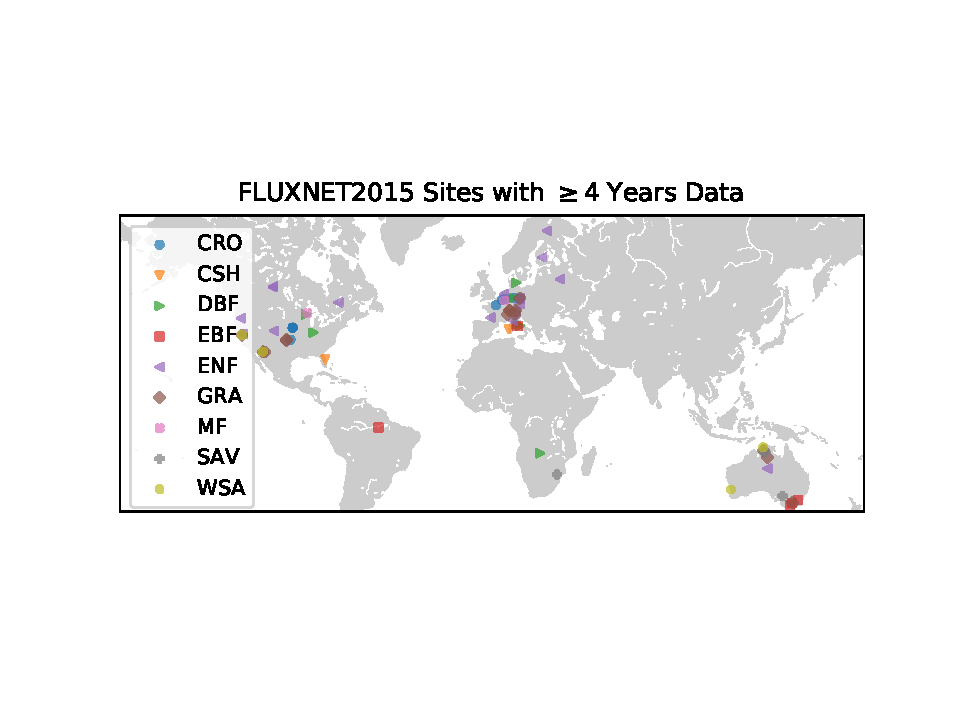
\includegraphics[width=\textwidth]{./map.pdf}
\caption{Plant functional type and location of FLUXNET2015 sites used
in this analysis.}
\label{map_fig}
 \end{figure}


The purpose of this study is to examine ecosystem response to
atmospheric drying, focusing on the growing season. To accomplish
this, we filter and quality control the data using a similar procedure
as \cite{Zhou_2015}:
\begin{itemize}
\item Only measured or highest (``good'') quality gapfilled data,
according to quality control flags, are used.
\item To isolate the growing season, we only use days in which the
average Gross Primary Productivity (GPP) exceeds 10\% of the observed
95th percentile of GPP for a given site. GPP is calculated using the
nighttime respiration partitioning method.
\item We remove days with rain and the day following to avoid issues
with rain interception and sensor saturation at high relative humidity
(\cite{MEDLYN_2011}).
\end{itemize} Additionally, as in \citet{Lin_2018}, we restrict data
to the daytime, which is identified when downwelling shortwave
radiation is greater than 50 W m$^{-2}$ and sensible heat flux is
greater than 5 W m$^{-2}$. To reduce the chance of sensor saturation
at high relative humidity, we remove all time steps for which VPD is
less than .01 kPa, and to reduce errors at low windspeeds we remove
all periods with wind magnitudes less than 0.5 m s$^{-1}$. Timesteps
with negative observed GPP or ET are also removed, and we aggregate
half hourly data to hourly averages to reduce noise
\citep{Lin_2018}. After these quality control procedures, 335,939
upscaled hourly observations remain.

\subsection{Methods}
\label{methods} The Penman-Monteith equation \citep [hereafter
PM,][]{Penman_1948, Monteith_1965} estimates ET as a function of
observable atmospheric variables and surface conductances:
\begin{linenomath*}
  \begin{equation}
    \label{orig_pen} ET = \frac{\Delta R_{net} + g_a \rho_a c_p
VPD}{\Delta + \gamma(1 + \frac{g_a}{g_s})},
  \end{equation}
\end{linenomath*} where $\Delta$ is the change in saturation vapor
pressure with temperature, given by Clausius-Clapeyron ($\frac{d \;
e_s}{d \; T}$), $R_{net}$ is the net radiation minus ground heat flux,
$g_a$ is aerodynamic conductance, $\rho_a$ is air density, $c_p$ is
specific heat of air at constant pressure, $\gamma$ is the
psychometric constant, and $g_s$ is the stomatal conductance (Table
\ref{definitions}).

\begin{table}
  \caption{Definition of symbols and variables, with citation for how
values are calculated, if applicable.}
  \label{definitions} \centering \small
\begin{tabular}{l c c c} \hline Variable & Description & Units &
Citation \\ \hline $e_s$ & saturation vapor pressure & Pa & - \\ $T$ &
temperature & K & - \\ $P$ & pressure & Pa & - \\ $\Delta$ &
$\frac{\partial e_s}{\partial T}$ & Pa K$^{-1}$ & - \\ $R_{net}$ & net
radiation at land surface minus ground heat flux & W m$^{-2}$ & - \\
$g_a$ & aerodynamic conductance & m s$^{-1}$ &
\citet{Shuttleworth_2012} \\ $\rho_a$ & air density & kg m$^{-3}$ & -
\\ $c_p$ & specific heat capacity of air at constant pressure & J
K$^{-1}$ kg$^{-1}$ & - \\ $VPD$ & vapor pressure deficit & Pa & - \\
$\gamma$ & psychometric constant & Pa K$^{-1}$ & - \\ $g_s$ & stomatal
conductance & m s$^{-1}$ & \citet{MEDLYN_2011} \\ $g_{l-s}$ &
leaf-scale stomatal conductance & mol m$^{-2}$ s$^{-1}$ &
\citet{MEDLYN_2011} \\ $R$ & universal gas constant & J mol$^{-1}$
K$^{-1}$ & - \\ $R_{air}$ & gas constant of air & J K$^{-1}$ kg$^{-1}$
& - \\ $LAI$ & leaf area index & -& - \\ $\sigma$ & uncertainty
parameter & -& - \\ $c_a$ & CO$_2$ concentration & $\mu$ mol CO$_2$
mol$^{-1}$ air& - \\ $\lambda$ & marginal water cost of leaf carbon &
mol H$_2$O mol$^{-1}$ CO$_2$ & - \\ $\Gamma$ & CO$_2$ compensation
point & - & - \\ $\Gamma^*$ & CO$_2$ compensation point without dark
respiration & - & - \\ \hline
\end{tabular}
\end{table}


\citet{MEDLYN_2011} developed a model for stomatal conductance ($g_s$)
by combining an optimal photosynthesis theory \citep{Farquhar_1980,
Katul_2010} with an empirical approach, which describes the dependence
of $g_s$ to VPD. This resulted in the following model for leaf-scale
stomatal conductance:

\begin{linenomath*}
  \begin{equation} g_{l-s} = g_0 + 1.6 \left(1 +
\frac{g_1}{\sqrt{VPD}}\right) \frac{A}{c_a}
  \end{equation}
\end{linenomath*} Where $g_1$ is a leaf-scale ``slope'' parameter, A
is the net CO$_2$ assimilation rate, and $c_a$ is the atmospheric
CO$_2$ concentration at the leaf surface. \cite{MEDLYN_2011} relate
the slope parameter ($g_1$) to physical parameters as:
\begin{linenomath*}
  \label{slope}
  \begin{equation} g_1 = \sqrt{\frac{3 \, \Gamma^* \,
\lambda}{1.6}},\footnote{Note this expression has units of of (mmol
mol$^{-1}$)$^{1/2}$, but this can be converted to Pa$^{1/2}$ using the
ideal gas law.}
  \end{equation}
\end{linenomath*}

where $\Gamma^*$ is the CO$_2$ compensation point for photosynthesis
(without dark respiration), and $\lambda$ is the marginal water cost
of leaf carbon ($\frac{\partial \; \text{transpiration}}{\partial \;
A}$). So, $g_1$ is a leaf-scale term reflecting the tradeoff of water
for carbon uptake and growth. The higher $g_1$, the more open the
stomata and the more they release water in exchange for carbon.

The Medlyn model for stomatal conductance has been shown to behave
very well across PFTs \citep[][]{Lin_2015}, and can be adapted to the
ecosystem scale by multiplying $g_{l-s}$ by leaf area index (LAI) and
converting units to m s$^{-1}$ with the ideal gas law:

\begin{linenomath*}
  \begin{equation} g_s = \text{LAI} \frac{R \,T}{P} \left( g_0 + 1.6
\left(1 + \frac{g_1}{\sqrt{VPD}}\right) \frac{A}{c_a}\right)
      \label{medlyn}
  \end{equation}
\end{linenomath*}

While Equation 3 can be used in PM (Equation 1), it will make
analytical work with the function intractable because $A$, net CO$_2$
assimilation rate, is functionally related to ET itself. To remove the
dependence of ET on $A$ we use fundamental semi-empirical results of
\citet{Zhou_2015}, who showed that the underlying Water Use Efficiency
(uWUE):

\begin{linenomath*}
  \begin{equation} uWUE = \frac{GPP \cdot \sqrt{VPD}}{ET}
    \label{uwue}
  \end{equation}
\end{linenomath*} is relatively constant across time and moisture
conditions within a plant functional type. If, following
\citet{Lin_2015}, we approximate $g_0$ as $0$ (i.e. we neglect
cuticular and epidermal losses - a reasonable assumption except in
very dry conditions), we can use uWUE to remove the $A$ dependence
from $g_s$ in a way that makes the PM equation analytically tractable:

\begin{linenomath*}
  \begin{equation} g_s = \frac{R \, T}{P} 1.6 \left(1 +
\frac{g_1}{\sqrt{VPD}}\right) \frac{uWUE \; ET}{c_a \; \sqrt{VPD}}.
    \label{new_g_s}
  \end{equation}
\end{linenomath*}

Note that uWUE is fit on the ecosystem scale as in \citet{Zhou_2015},
so GPP in Equation \ref{uwue} is really $A \cdot \text{LAI}$. This
leads to the cancellation of LAI in the step from Equation
\ref{medlyn} to Equation \ref{new_g_s}. Plugging Equation
\ref{new_g_s} into Equation \ref{orig_pen} and rearranging gives a new
explicit expression for PM, in which dependence on $A$ is removed:

\begin{linenomath*}
  \begin{equation} ET = \frac{\Delta R_{net} + \frac{g_a\; P}{T}
\left( \frac{ c_p VPD}{R_{air}} - \frac{\gamma c_a \sqrt{VPD} }{ R \;
1.6\; \text{ uWUE } (1 + \frac{g_1}{\sqrt{VPD}})} \right) }{ \Delta +
\gamma}
    \label{et}
  \end{equation}
\end{linenomath*}

With Equation \ref{et}, ET is explicitly a function of environmental
variables and two plant-specific constants, the slope parameter
($g_1$), and uWUE, both reflecting water conservation strategy. The
slope parameter is a leaf-scale term related to the willingness of
stomata to trade water for CO$_2$ and to keep stomata open. uWUE is a
semi-empirical ecosystem-scale constant related to how WUE changes
with VPD (specifically $VPD^{-1/2}$). Is is also roughly proportional
to physical constants:

\[uWUE \appropto \sqrt{\frac{c_a - \Gamma}{1.6 \lambda}},\]

where $\Gamma$ is the CO$_2$ compensation point \citep[Equation 5
in][]{Zhou_2014}. So uWUE is related to atmospheric CO$_2$
concentration and compensation point, and is inversely proportional to
the marginal water cost of leaf carbon.

Given eddy-covariance FLUXNET2015 data (Section \ref{data}), every
term in our new version of PM (Equation \ref{et}) is observed, except
for the two parameters $g_1$, and uWUE. $g_1$ has been measured and
reported for the PFTs considered here \citep{Lin_2015, Franks_2017},
and we fit uWUE by calculating its expectation, given the model and
FLUXNET2015 data.

However, eddy-covariance data are inherently noisy so we include a
measure of uncertainty in our analysis. To account for observational
error, as well as model uncertainty (e.g. temporal and spatial
variations of uWUE), we introduce an uncertainty parameter $\sigma$
modifying uWUE:

\begin{linenomath*}
  \begin{equation} ET = \frac{\Delta R_{net} + \frac{g_a\; P}{T}
\left( \frac{ c_p VPD}{R_{air}} - \frac{\gamma c_a \sqrt{VPD} }{ R \;
1.6\; \sigma \; \text{ uWUE } (1 + \frac{g_1}{\sqrt{VPD}})} \right) }{
\Delta + \gamma}
    \label{et_sigma}
  \end{equation}
\end{linenomath*}

Now, from each FLUXNET2015 observation (i.e. for each hourly
observation at every time step) we can evaluate $\sigma$:

\begin{linenomath*}
  \begin{equation} \sigma = - \frac{g_a \gamma c_a \sqrt{VPD} L_v P }{
\left(\text{ ET } ( \Delta + \gamma) - \Delta R_{net} - g_a \rho_a c_p
VPD\right) 1.6 \; R\; T\; \text{ uWUE } (1 + \frac{g_1}{\sqrt{VPD}})},
    \label{sigma}
  \end{equation}
\end{linenomath*}

Thus, with this uncertainty analysis we can evaluate departure from
our theory in observations, as a departure of $\sigma$ from unity. The
variability of $\sigma$ across sites and time provides a measure of
uncertainty in our model, assumptions, as well as in the FLUXNET2015
observations themselves. The variability of $\sigma$ then propagates
through any uncertainty to our derivative of Equation \ref{et_sigma}:

\begin{linenomath*}
  \begin{equation} \frac{\partial \; ET}{\partial \; VPD} = \frac{2\;
g_a \; P}{T(\Delta + \gamma)} \left(\frac{ c_p}{R_{air}} -
\frac{\gamma c_a }{1.6 \; R\; \sigma \; \text{ uWUE }} \left( \frac{2
g_1 + \sqrt{VPD}}{2 (g_1 + \sqrt{VPD})^2}\right) \right)
    \label{d_et}
  \end{equation}
\end{linenomath*}

With Equation \ref{d_et} we have an analytical framework for ecosystem
response to atmospheric demand perturbations, with an implicit
assumption of non-extreme drought conditions. There are a few
subtleties to taking the derivative in Equation \ref{d_et}: $\Delta$
($\frac{d e_{s}}{d T}$) and $VPD$ are functionally related, so while
taking the derivative we evaluate $\frac{\partial \; ET}{\partial \;
VPD} = \frac{\partial \; ET} {\partial \; e_s} \frac{\partial \;
e_s}{\partial \; VPD} \Big|_{\text{RH fixed}} + \frac{\partial \;
ET}{\partial \; RH} \frac{\partial \; RH}{\partial \; VPD}
\Big|_{\text{$e_s$ fixed}}$. $RH$ and $e_s$ are assumed to be
approximately independent, which is supported by the data (not shown).

We note one final comment on our derivation which is relevant for
drought indices. If we approximate $c_a$ at a global mean CO$_2$
concentration, then the RHS of Equation \ref{et} is fully defined
using commonly available weather station data and the constants
published in \citet{Zhou_2015} and \citet{Lin_2015}. This makes
Equation \ref{et} a useful alternative to PET in drought indices and
hydrometeorological analysis for vegetated surfaces. Equation \ref{et}
better reflects the physics of water exchange at the land surface and
would only require fitting of uWUE and $g_1$, and can also account for
changes in CO$_2$ concentration, contrary to typical drought indices
such as the Palmer Drought Severity Index (PDSI) \citep{Swann_2016}.




\section{Results}
\label{results}

By construction, the variability in the $\sigma$ term (Equation
\ref{sigma}) contains all model and observational uncertainties. For
an observation that perfectly matches our model and constant uWUE
assumption, $\sigma$ will be one. Therefore, for our assumptions and
framework to be reasonable $\sigma$ should be close to 1. An
additional concern is that $\sigma$ may in fact be correlated with
$VPD$, in which case the dependence would need to be accounted for
when taking the derivative. Fortunately, there is a very weak
dependence of $\sigma$ on VPD in their joint distrubution, and
$\sigma$ is indeed close to unity i.e. $O(1)$ (Figure
\ref{joint_vpd_sigma}). Given this weak dependence and the
distribution of $\sigma$ we have confidence in our model framework and
the data quality.

\begin{figure} \centering
\includegraphics[width=\textwidth]{./joint_vpd_sigma.pdf}
\caption{The joint distribution of $VPD$ and $\sigma$, with outliers
removed (defined as lowest and highest 5\% of $\sigma$). $\sigma$
exhibits a weak dependence on $VPD$, and $\sigma$ is $O(1)$ for the
bulk of the observations.}
\label{joint_vpd_sigma}
\end{figure}

Before calculating the sensitivity of ET to VPD, we will consider the
functional form of Equation \ref{d_et}. There are two main terms: a
``scaling'' term, which modifies the magnitude but not the sign of the
ET response to VPD ($\frac{\partial \; ET}{\partial \; VPD}$):

\begin{equation} \frac{g_a \; P}{T(\Delta + \gamma)},
\end{equation}

and a ``sign'' term, which determines whether ET increases or
decreases with VPD (i.e. atmospheric demand driven or physiologically
controlled):

\begin{equation}
  \label{sign} \frac{c_p}{R_{air}} - \frac{\gamma c_a }{1.6 \; R\;
\text{ uWUE }} \left( \frac{2 g_1 + \sqrt{VPD}}{2 (g_1 +
\sqrt{VPD})^2}\right).
\end{equation} All variables are positive, so the relative magnitude
between the first term and the second term in the sign term (Equation
\ref{sign}) will determine whether ET increases or decreases with
increasing VPD. If the second term is larger then plant control
dominates and ET decreases with increasing VPD. However, if the first
term is larger, then atmospheric demand dominates and ET increases
with increasing VPD.

\subsection{Functional Form of the Sign Term}
\label{sign_term} First, we explore the variables within the sign term
to gain better intuition on the driver of either the increase or
reduction of ET with VPD. CO$_2$ concentration ($c_a$) and the
psychometric constant ($\gamma$) are relatively constant over the
dataset considered here so that the variability is dominated by
$\sigma$ and $VPD$. uWUE could vary with soil moisture but has been
shown to be relatively constant \citep{Zhou_2015}. This then means
that the sign term only depends on VPD for a given PFT and is
approximately just a function of $VPD$. We can further determine a
critical threshold separating an increase from a decrease in ET,
i.e. the threshold $VPD_{crit}$ such that the derivative vanishes
$\frac{\partial \; ET}{\partial \; VPD} = 0$: \small
\begin{linenomath*}
  \begin{equation} VPD_{crit} = \frac{R_{air}}{4 c_p} \left(
\frac{\gamma c_a}{1.6\; R \; uWUE} + \sqrt{\frac{\gamma c_a}{1.6\; R
\; uWUE}\left( \frac{\gamma c_a}{1.6\; R \; uWUE} + 8 g_1
\frac{c_p}{R_{air}}\right)} - 4 g_1 \frac{c_p}{R_{air}} \right),
\label{vpd_min_et}
  \end{equation}
\end{linenomath*} \normalsize noting that $VPD_{crit}$ mostly depends
on the PFT parameters uWUE and $g_1$, and only varies weakly with
climate as most other parameters related to the environment are nearly
constant. The calculated value of $VPD_{crit}$ for each PFT is shown
in Table \ref{vpd_crit}. For any values of $VPD$ less than
$VPD_{crit}$, ET will thus decrease with increasing VPD
($\frac{\partial \; ET}{\partial \; VPD} < 0$), and for values of
$VPD$ greater than $VPD_{crit}$, ET will increase with increasing VPD
($\frac{\partial \; ET}{\partial \; VPD} > 0$). In other words,
ecosystems regulate and mitigate evaporative losses up to the VPD
limit, $VPD_{crit}$, above which atmospheric demand is just too high
to be entirely compensated by stomatal and ecosystem regulation. We
note however that even though ET increases again above the critical
threshold, $VPD_{crit}$, ET is still much lower that potential
evaporation as stomata are still strongly regulating vapor fluxes to
the atmosphere. Indeed, even in the absence of soil pore evaporation,
stomata do not shut down entirely at very high VPD so that ET does not
go to zero, because stomata are still slightly open to perform some
photosynthesis \citep{Ball_1987, Leuning_1990, MEDLYN_2011}. In
addition, upward xylem transport is necessary to maintain phloem
transport, as well as nutrient transport and thus carbon allocation
\citep{De_2013, Nikinmaa_2013, Ryan_2014}.



\begin{table}
\caption{Values of $VPD_{crit}$, where $\frac{\partial \; ET}{\partial
\; VPD} = 0$, evaluated at PFT average values for $R_{air}$, $\gamma$,
and $c_a$. PFT-specific constants ($g_1$, uWUE) are provided in Table
\ref{pft}. For values of $VPD$ less than $VPD_{crit}$, $\frac{\partial
\; ET}{\partial \; VPD}$ will be negative, and for values of $VPD$
greater than $VPD_{crit}$, $\frac{\partial \; ET}{\partial \; VPD}$
will be positive.}  \centering
\begin{tabular}{l c c c c c} \hline PFT & $R_{air}$ & $c_a$ (ppm) &
$\gamma$ & \textbf{$VPD_{crit}$ (Pa)} \\ \hline CRO & 288.6 & 376.0 &
65.2 & \textbf{936.6} \\ CSH & 289.0 & 383.6 & 67.5 & \textbf{12852.5}
\\ DBF & 288.6 & 379.5 & 63.6 & \textbf{1266.6} \\ EBF & 288.4 & 368.5
& 61.6 & \textbf{1454.8} \\ ENF & 288.28 & 379.8 & 61.0 &
\textbf{1853.7} \\ GRA & 288.4 & 378.0 & 61.0 & \textbf{3261.1} \\
\hline
\end{tabular}
\label{vpd_crit}
\end{table}


Differences in $VPD_{crit}$ are exclusively determined by uWUE and the
slope parameter ($g_1$) related to the plant functional type. A larger
uWUE means a smaller $VPD_{crit}$, and an ET response to increases VPD
that is more likely to be positive. At first glance this result is
somewhat counter-intuitive; we expect that plants with a higher water
use efficiency would be more water conservative. However, in reality
uWUE determines how $WUE$ changes with VPD:

\[WUE = \frac{GPP}{ET} = \frac{uWUE}{\sqrt{VPD}}.\]
\[\frac{\partial \; WUE}{\partial \; VPD} = -\frac{uWUE}{2 \;
VPD^{3/2}}\]

So, plants with a higher uWUE will have a greater \textit{decrease} in
ecosystem-scale $WUE$ in response to increases in VPD. This decrease
in $WUE$ causes more water loss per unit carbon production, and
explains the relationship between high uWUE and high likelihood of
increases of ET in response to increasing atmospheric drying
(increases in VPD).

A tendency towards increasing ET response with increasing VPD can also
be caused by a high slope parameter ($g_1$), characteristic of plants
that at the leaf scale are more willing to trade water for access to
atmospheric CO$_2$. Plants that are less conservative will be thus be
more likely to increase ET with increasing VPD. Both the
aforementioned effects (large uWUE, $g_1$) can amplify each other, and
generally conspire to shift the sign term towards a positive value for
a given PFT.

This effect of uWUE and $g1$ on the sign term is most apparent by
comparing two extreme PFTs: water intensive crops (CRO) and water
conservative closed shrub (CSH). CRO has high slope parameters and
uWUE ($g_1 = 183.1$ Pa$^{1/2}$; $2.27$ $\mu$-mol [C] Pa$^{0.5}$
J$^{-1}$ [ET]) compared to CSH ($g1 = 148.6 \, Pa^{1/2}$, $uWUE=1.66$
$\mu$-mol [C] Pa$^{0.5}$ J$^{-1}$ [ET]). These differences in PFT
parameters cause opposite ET responses to changes in VPD between CRO
and CSH. ET theoretically always decreases with increasing VPD for the
more water conservative CSH, while ET frequently increases with
increasing VPD for the more water intensive CRO (Figure
\ref{idealized_sign}). CRO evolved or were bred to prioritize GPP and
yield and are thus not water conservative. They are very willing to
trade water for photosynthesis and productivity, despite changes in
VPD, while CSH are very unwilling to trade water for more
photosynthesis.

\begin{figure} \centering
\includegraphics[width=\textwidth]{./idealized_sign.pdf}
\caption{The functional form of the sign term, with $\sigma$ held
fixed at 1, and all terms except VPD set to PFT averages. For
comparison, the observed range of VPD for each PFT is plotted below
the x-axis. Stars denote 25th, 50th, and 75th percentiles, and the
range of the line spans the 5th-95th percentiles of observed
VPD. Vertical black lines denote the location of $VPD_{crit}$ for each
PFT, with the exception of CSH, for which $VPD_{crit}$ is off-scale.}
\label{idealized_sign}
\end{figure}


As expected, the slope parameter ($g_1$) is a primary determinant of
the VPD dependence for the sign term shown in Figure
\ref{idealized_sign}. Plants that are more conservative (small $g_1$)
will tend to reduce ET with increasing VPD, and will be very effective
at reducing ET, especially at low VPD. However, at very high VPD,
gradients in vapor pressure at the leaf scale will be so strong that
they will begin to dominate leaf-scale plant strategies of stomatal
(partial) closure (parameterized with $g_1$). As a result, ET response
will begin to asymptote towards its ecosystem-scale values
irregardless of leaf-scale strategy and stomatal regulation
(parameterized with $g_1$). Therefore, plants with a low $g_1$ will
have the largest VPD dependence of ET response because the difference
in ET response at low VPD (leaf stomatal response dominates) and high
VPD (VPD gradient dominates) is largest. This is apparent in the
strong VPD dependence of ENF, which has the lowest slope parameter
($g_1=74.31$ Pa$^{1/2}$) (Figure \ref{idealized_sign}).

To summarize our theoretical insights (Figure \ref{idealized_sign} and
Table \ref{vpd_crit}), CROs are the least water conservative and have
the strongest overall tendency to increase ET with increasing VPD,
while CSH are the most water conservative and have the strongest
tendency to decrease ET with increasing VPD.  ENF ($g_1 = 74.31$
Pa$^{1/2}$) has by far the largest VPD response dependence, while CRO
($g_1 = 183.1$ Pa$^{1/2}$) has the smallest VPD dependence. Figure
\ref{idealized_sign} clearly shows, according to our theory, that for
all PFTs except for crops there is frequent occurrence of a negative
(plant dominating) ET response to increases in VPD. Therefore, plants
are able in most atmospheric conditions to reduce ET in response to
increased VPD and thus to reduce water loss. To better illustrate
this, the ranges of observed environmental VPDs at the FLUXNET sites
are plotted parallel to the x-axis. For CSH, VPD is always less than
VPD$_{crit}$ (off scale) so that the plant response dominates in
typical environmental conditions, emphasizing the water conservative
strategy of those plants. For CRO on the other hand, VPD is higher
than VPD$_{crit}$ for more than 50\% of observations, emphasizing that
those plants operate with an aggressive water usage strategy, are
water intensive and were actually engineered for photosynthesis rather
than water saving. For forests and grass, more than half of the
observed VPD are less than VPD$_{crit}$, i.e. in conditions where
plant response dominates. It is also important to note that even when
atmospheric demand dominates, ET response to VPD is still far more
negative than it would be for potential evaporation $\partial
PET/\partial VPD$, i.e. atmospheric demand only, emphasizing that
there is still a strong regulation of evaporative flux by stomata and
though the plant xylem. The sign term in the PET case would just be a
constant ($\frac{c_p}{R_{air}} \approx 3.5$), which is far larger than
any part of the curves for any PFT. This highlights the deficiencies
of PET's ability to capture land response to changes in atmospheric
dryness (VPD). Plants are always regulating water exchange from the
land surface, even when they reach the limits of they ability to do
so.

\subsection{Functional Form of the Scaling Term}
\label{scale_term} While the above discussion of the sign of
$\frac{\partial \; ET}{\partial \; VPD}$ is important to answer our
question of when ET response increases or decreases with VPD,
understating the overall magnitude of the ET response is important to
soil-plant-atmosphere water budgeting. So we now more closely examine
the terms that affect how the sign term is scaled:

\begin{equation} \frac{g_a \; P}{T(\Delta + \gamma)}:
\end{equation}

$\frac{P}{T}$ is an air-density term, which varies little compared to
aerodynamic conductance and Clausius-Clapeyron ($\Delta$). The
psychometric constant ($\gamma$) is also relatively constant, so the
scaling term should be primarily a function of aerodynamic conductance
and temperature, through the Clausius-Clapeyron relationship
$\Delta$. This is as expected, given that the aerodynamic conductance
represents the efficiency of exchange between the surface and the
atmosphere. As aerodynamic conductance increases, any plant response
will be communicated more strongly to the atmosphere (and vice-versa).

$\Delta$'s presence in the scaling term also matches physical
intuition. $\Delta$ (and also the approximately constant $\gamma$)
control the efficiencies with which surface energy is converted to
latent and sensible heat \citep{Monteith_1965}. The functional from of
$\Delta$ will be the same across PFTs, but the temperature range may
vary slightly. In contrast, aerodynamic conductance will vary strongly
with PFT due to the importance of surface roughness for aerodynamic
conductance. So most of the differences in scaling between PFT should
be in the aerodynamic conductance term.

The control of the scaling term variability between PFTs by
aerodynamic conductance is confirmed by data (Figure
\ref{scale_vary}). Differences between PFT are almost entirely due to
differences in aerodynamic conductance, rather than differences in
observed temperature ranges. The scaling term for the tree PFTs (DBF,
EBF, ENF) is generally about double the scaling terms for the other
PFTs which have lower surface roughness and generally smaller
aerodynamic conductance.

\begin{figure} \centering
\includegraphics[width=\textwidth]{./idealized_scale.pdf}
\caption{Primary sources of variability for the scaling term, as a
function of PFT. The 5th-95th percentile range of temperature is
plotted at the 5th, 25th, 50th, 75th, and 95th percentiles of
aerodynamic conductance, as observed for each PFT.}
\label{scale_vary}
\end{figure}

Within each PFT, the scaling term variability is controlled both by
environmental temperature and aerodynamic conductance variability
(Figure \ref{scale_vary}). While the observed variability of the
aerodynamic conductance contributes more to the scaling term
variability than temperature, the temperature contribution is
non-negligible. Specifically, the scaling term is generally larger at
low temperatures when latent heat is relatively inefficient at moving
energy away from the surface. This effect amplifies the role of
aerodynamic conductance variability at low temperatures.

To summarize, variability between PFTs is mostly controlled by
systematic differences in aerodynamic conductance, due to differences
in surface roughness between each PFT, and possibly to a lesser extent
wind conditions. In contrast, variability within PFT is also
controlled by temperature, through Clausius-Clapeyron. But,
aerodynamic conductance variability generally impacts the scaling term
more than temperature, even within PFT.

\subsection{Bulk statistics of ET response to VPD}
\label{stats_sec}

In this section we consider direct observations of ET response with
eddy-covariance data, while including uncertainty with the $\sigma$
term (Section \ref{methods}). These observational results of ET
response largely confirm our theoretical analysis, presented above
(Table \ref{stats}). For all PFTs, mean ET response to increasing VPD
is negative. However, ET response evaluated at the average of all
variables (e.g. $\sigma$, $T$, $c_a$, $VPD$) is positive for CRO, and
negative for all other PFTs. This difference in mean ET response as
compared to the ET response at mean environmental conditions is due to
the non-linear nature of the response, in which negative responses are
generally larger magnitude than positive responses (Figure
\ref{idealized_sign}). Therefore, both the mean ET response as well as
the ET response at mean environmental conditions matches our
expectations from the theory (Section \ref{sign_term}), with the
exception that CRO observations are shifted more towards a negative ET
response than we expect.

\begin{table}
\caption{Statistics of $\frac{\partial \; ET}{\partial \; VPD}$ as a
function of PFT.}  \centering
\begin{tabular}{l c c c} \hline PFT & $\overline{\frac{\partial \;
ET}{\partial \; VPD}}$ & $\frac{\partial \; ET}{\partial \;
VPD}\left(\overline{env}\right)$ & fraction $\frac{\partial \;
ET}{\partial \; VPD} < 0.$ \\ \hline CRO & -0.05 & 0.008 & 0.533 \\
DBF & -0.10 & -0.013 & 0.609 \\ EBF & -0.13 & -0.037 & 0.666 \\ GRA &
-0.07 & -0.024 & 0.694 \\ ENF & -0.17 & -0.081 & 0.740 \\ CSH & -0.29
& -0.224 & 0.973 \\ \hline
\end{tabular}
  \label{stats}
\end{table}

Regarding the frequency of negative and positive ET response, all PFTs
exhibit a decreasing ET response with increasing VPD (physiologically
controlled, water conservative response) for the majority of
observations. When listed by increasing frequency of negative
response, the PFTs are generally ordered as we would expect them to
be, from most water intensive to most water conservative: CRO (53\%),
DBF (61\%), EBF (67\%), GRA (69\%), ENF (74\%), and CSH (97\%).

In general the bulk statistics match our theoretical expectations
well, with the caveat that inclusion of uncertainty shifts crops
towards a slightly more negative response than the theory and Figure
\ref{idealized_sign} would suggest. The bulk statistics motivate a
more thorough examination of the structure of uncertainty and more
sophisticated validation of our theory's performance against
observations.

\subsection{Validation of theory at eddy-covariance sites}
\label{testing} We now compare more sophisticated distributions of the
observed response to our simplified theory (Section
\ref{sign_term}). The observed distribution of the sign term, as
compared to what the theory would predict, is provided in Figure
\ref{test_sign}. Our goal was to capture the leading order behavior of
the ET dependence on VPD. Given the assumptions we have made, and the
uncertainties of flux tower observations themselves, we expect a
relatively large amount of noise when reproducing the derivatives of
ET. However, the data largely reproduces our theoretical analysis.

\begin{figure} \centering
\includegraphics[width=\textwidth]{./test_sign.pdf}
\caption{Comparison of the sign term with model uncertainty included
(box plots) to the sign term as calculated with simplifying
assumptions (blue line, as in Figure \ref{idealized_sign}). Each box
plot corresponds to 5\% of the data, and the 5-95\% range of VPD is
plotted.}
\label{test_sign}
\end{figure}

For DBF our theory is successful towards this goal: the theory matches
the leading order behavior of the function when uncertainty is
included, and the observations match the theory with the addition of
noise. The VPD dependence, given by the slope parameter ($g_1$),
follows the median values of each bin. Perhaps most importantly, the
x-intercept, and thus VPD$_{crit}$, matches nearly exactly between the
theory and the observations. Therefore the sign of the ET response to
increases in VPD should be well matched, subject to the unavoidable
constraints of noise, much of which comes from the observations
themselves. The uncertainty is non negligible; there are many
observations in each bin for which the the sign of observation is
opposite the response predicted by the theory, but to leading order
our theory matches the observations well.

While CSH has a much different functional form of the sign term than
DBF, CSH observations also match our theory to leading order. Again,
the VPD dependence mostly determined from the slope parameter ($g_1$)
closely matches the medians in the observation bins and the
theoretical threshold is well reproduced (albeit off-scale). The
VPD-independent, strongly negative response, which is determined by
uWUE, is also captured. For CSH, there is extremely rare occurrence of
observed positive ET response with VPD ($\approx 3$\%), even with
uncertainty, so the sign of the observations almost always matches the
sign of the theory, which states that ET response should always be
negative.

As Table \ref{stats} suggested, the theory does not match as well for
CRO as for DBF and CSH. At low VPD the VPD dependence (due to $g_1$)
is similar to the leading order behavior of the observations, but the
theory's curve is shifted towards more positive values relative to the
observations, likely due to some bias in uWUE. Most strikingly, the
observations show a tendency to move back towards negative values at
high VPD, which given the functional form of VPD dependence, is
behavior that is impossible for the theory to capture. This general
positive bias of the theory explains the shift towards negative ET
response observed in the bulk statistics in Table \ref{stats}. The
divergence between the theory and the observations for CRO could have
been expected. For practical reasons, our theory does not include
important sources of plant type heterogeneity within and across sites
for CRO. In agricultural landscape, the footprint of an
eddy-covariance towers tend to not only observe a single species but
many different ones, with potentially varying water use strategies. We
also do not account for seasonal changes in LAI, variability in crop
height and surface roughness, differences in C3 vs C4 photosynthesis
and water strategies, or differences in irrigation practices between
the sites and years. These deficiencies should largely explain the
inability of our theory to exactly match the observations in
croplands. For example, a superposition of sites with C3 plants (at
low environmental VPD) and C4 plants (at high environmental VPD) would
explain observed shift back towards negative ET response at high VPD
when all sites are binned together, as in Figure \ref{test_sign}.

The theory for GRA suffers from similar limitations as for CRO. GRA
observations are characterized by a consistent trend back towards
negative ET response at higher VPD, which the functional form of our
theory is incapable of accounting for. As compared to CRO, the
divergence between the theory and the observations is even greater for
GRA, but these differences are explainable using similar logic as we
did for CRO. GRA also tends to exhibit substantial within-PFT
variability, such as C3 vs C4 photosynthesis, as well as strong
seasonal variability in height and LAI. As with CRO, the trend back
towards negative ET response at higher VPD could be explained by a
superposition of sites with C3 vs C4 plants. Unfortunately, because
detailed site-level data of C3 vs C4 plant type is not available, we
could not bin CRO and GRA further by irrigation and photosynthesis
strategy. However, we hypothesize that the theory would validate
against observations much better when photosynthesis pathways are
accounted for.

The comparison between the theory and observations for ENF and EBF is
unique from the rest of the PFTs. The VPD dependence of the theory,
determined by the slope parameter ($g_1$), is not as well captured by
observations. However, the theory still captures the general behavior
and magnitude of the response, with some increase in error at low
and/or high VPD.  We note that we used published constants for $g_1$
\citep[from ][]{Lin_2015, Franks_2017}, which determines the VPD
dependence, and that deviations should be expected across sites
\citep{Lin_2015}. We could have fit our own constants so that the
theory would best match the observations, but our goal was to use a
priori results whenever possible in order to avoid over-fitting and to
have a theoretical approach as independent to the observations as
possible for further confirmation of the validity of the approach.

While the above discussion shows that our theory has some limitations
when applied to some PFTs, especially for crops and grasslands, it
does well for DBF and CSH PFTs, and captures the response at
non-extreme VPD for ENF and EBF. It is useful to also compare our
theory, the observed uncertainty in the ET response, and PET, as PET
is often used as a proxy for ET in hydrometeorological studies and
drought indices. Again, as in our discussion of the theoretical
results, the PET sensitivity to VPD will be constant at about 3.5. In
Figure \ref{test_sign} the ET response to shifts in dryness is always
far smaller than 3.5 in the observations, even with all uncertainty
included. So the PET response to atmospheric dryness is outside the
range of all observable responses. This casts doubt on PET's
usefulness for capturing the leading order behavior of water budget
and dryness response at the land surface, as is done in several
drought indices. However our theory (Equation \ref{et}) could be used
with published uWUE and $g1$ data, as an alternative to PET to
estimating land response and dryness, and would more accurately
account for the response to atmospheric drying.

\subsection{Observed ET response to VPD}

Most of the results presented so far focus on the sign term, so now we
turn to observations of ET response with the scaling term included
(Figure \ref{data_scatter}). Until now, in the interest of developing
leading order intuition for ET response, and to be conservative in our
acknowledgment of model and observational error, we've considered
$\sigma$ variability to be a measure of uncertainty. An alternative
viewpoint is that $\sigma \cdot uWUE$ represents spatial and temporal
variability of uWUE, which may be expected within bounds \citep[see
Table \ref{pft}, also ][]{Zhou_2015}. This is a less conservative
view; some of the $\sigma \cdot uWUE$ variability will be due to model
and observational error, so by viewing $\sigma \cdot uWUE$ as
\textit{real} variability we run the risk of mistaking noise for
signal. However, the advantage of this viewpoint is that, from
\citet{Zhou_2014}, we have very high confidence that uWUE fit at the
hourly timescale (as we do with $\sigma \cdot uWUE$) correctly
captures the relationship between ET, GPP, and VPD, and that our form
of PM introduces minimal error with its use of uWUE.

\begin{figure} \centering
\centerline{\includegraphics[width=\textwidth]{./data_scatter.png}}
\caption{Scatter plots of observed $\frac{\partial \; ET}{\partial \;
VPD}$, including $\sigma$ variability, as a function of PFT,
temperature and VPD. Please note differences in the colorbar scale.}
\label{data_scatter}
\end{figure}

Therefore, with the caveat that some of the signal presented in Figure
\ref{data_scatter} may in fact be noise, we can interpret the observed
distribution of ET response to VPD. In general, the observed response
matches the intuitive theory. ET response to VPD shifts towards
positive values as VPD increases (atmospheric demand dominating). CRO
exhibit the highest occurrence of positive ET response, and the
observations confirm that CRO are the most water intensive. CSH are
the most water conservative, with a strong negative response. DBF,
EBF, ENF, and GRA are also water conservative, but show some
occurrence of positive ET response to VPD, particularly at higher
observed VPD, as the theory predicts.

Figure \ref{data_scatter} also includes the impact of the scaling
term. For a given VPD, the magnitude of ET response does not vary
strongly with temperature, confirming that any impact of the scaling
term on the magnitude of the response is primarily due to changes in
aerodynamic conductance. Intuitively this is reasonable; aerodynamic
conductance will control how dominant balances at the land surface are
communicated to the boundary layer. While $\Delta$ controls the
efficiency of energy conversion to latent heat, it appears this is a
second order term, relative to $g_a$, for scaling ET response.

As in Figure \ref{test_sign}, Figure \ref{data_scatter} matches our
expectation based on simplified theory. The sign term is most strongly
scaled by $g_a$, and in general the sign term shifts towards positive
values as VPD increases. The willingness with which a given plant type
evolved to use water dictates the occurrence of positive versus
negative ET response. Water conservative plants are highly effective
at mitigating the effects of atmospheric demand, and can store water
for later use by reducing ET in response to increasing VPD.

\subsection{Limitations of theory - very dry soil moisture conditions}
In formulating our theory with Penman Monteith, we implicitly did not
account for very dry soil moisture conditions. For the majority of
environmental conditions observed at the eddy covariance sites used
here, soil conditions were not extremely dry so that we could assume a
constant uWUE and $g_1$. We posit that ecosystems will generally
optimize to host plants living in conditions which they evolved
for. However, in extreme conditions and drought scenarios soil water
content (SWC) could become the limiting factor for ET response to VPD,
which our theory does not account for. In addition, low soil moisture
conditions themselves increase VPD through land-atmosphere feedback
\citep[][]{Bouchet_1963, Morton_1965, Brutsaert_1999, Ozdogan_2006,
Salvucci_2013, Gentine_2016, Berg_2016}.

We first note that in the data used low SWC conditions are very
infrequent. Within our framework, any systematic bias due to the
failure to account for SWC's effects in very dry conditions should
manifest itself in a functional relationship between $\sigma$, our
uncertainty measure, and SWC, which is observed at the FLUXNET
sites. Examining the relationship between $\sigma$ and SWC will test
to what extent our theory breaks down in very dry soil moisture
conditions.

If we again view $\sigma \cdot uWUE$ as, in addition to a measure of
uncertainty, a short time-scale observation of uWUE, we would expect
$\sigma \cdot uWUE$ to decrease at low SWC. If $\sigma \cdot uWUE$ is
a very strong function of SWC, then our theory should be conditioned
more strongly on well watered soil conditions. If $\sigma \cdot uWUE$
is weakly a function of SWC, then our theory is more universal and
independent of soil moisture conditions.

Indeed, for all PFTs, there is some slight dependence of $\sigma \cdot
uWUE$ on SWC, especially at low SWC (Figure \ref{swc_boxplot}). The
portion of observations for which our theory is biased by
SWC-limitations varies by PFT, due to the nonlinear threshold at which
soil moisture availability limits plant function. For CRO and DBF,
soil water content only matters for about the lowest 5\% of
observations (each box is 5\% of observations in Figure
\ref{swc_boxplot}). And, CRO, relative to DBF, has a very weak
dependence on soil moisture, which is reflective of the high
likelihood that CRO sites are optimally irrigated and not water
stressed. For ENF and EBF, systematic SWC-induced biases in $\sigma
\cdot uWUE$ emerge in about the lowest 30\% of SWC conditions. In
crontast to ENF, CRO, and DBF, for GRA the relationship between
$\sigma \cdot uWUE$ and SWC is more linear and affects a greater
portion of observations; about 60\% of observations. Clearly, for GRA
soil water frequently impacts plant function and alters ET response,
and our theory is limited. It is therefore not suprising that our
theory tested poorly againt the data for GRA, relative to ENF, EBF,
DBF, and CSH (Section \ref{testing}). For all other PFTs occurence of
soil mosture impacts was rare enough to not manifest itself in bulk
statistics and plots. A possible exception is CSH, for which there are
only two sites, which precludes comment on the exact PFT-wide
relationship.

\begin{figure} \centering
\includegraphics[width=\textwidth]{./swc_boxplot.pdf}
\caption{$\sigma \cdot uWUE$ as a function of PFT and SWC. Each box
plot represents 5\% of all observations.}
\label{swc_boxplot}
\end{figure}

The observed dependence of $\sigma \cdot uWUE$ on SWC for GRA would
explain the deficiencies of our theory compared to the observations in
Figure \ref{idealized_sign}, specifically the trend back towards
negative soil moisture at high VPD. Aforementioned feedbacks between
the land surface and the atmosphere, which are not accounted for due
to our focus on the one-way response of the land surface to
atmospheric conditions, would cause high VPD to be correlated with low
SWC \citep[][]{Gentine_2016, Berg_2016}. So, at high VPD observations
of low SWC are more likely, and this low SWC causes a lower uWUE
(Figure \ref{swc_boxplot}). The lower uWUE at low SWC/high VPD then
leads to the observed downturn towards decreasing ET with increasing
VPD, and the deviation between our theory (based on a constant uWUE
assumption) and observations.

To summarize, our theory is limited by its inability to account for
soil water impacts on land surface response, and feedbacks between SWC
and VPD. Fortunately, for most PFTs SWC's effect on ET is relatively
rare (<30\% of observations) and does not manifest itself in the
majority of observations and bulk statistics. However, for GRA SWC has
a strong effect decreasing water use efficiency for the majority of
the observations. Soil moisture effects explain the deficiencies of
our theory in Section \ref{testing}, particularly for GRA.

\section{Discussion}

We derived a new form of Penman Monteith using the concept of
semi-empirical optimal stomatal regulation \citep{Lin_2015,
MEDLYN_2011} and near constant uWUE \citep{Zhou_2015} to remove the
implicit dependence of stomatal conductance on GPP and ET. With our
new form of Penman Monteith we developed a theory for when an
ecosystem will tend to reduce or increase ET with increasing VPD,
which we evaluated against a range of eddy-covariance data spanning
different climates and plant functional types. The goal was to capture
the leading order behavior of the system to gain some intrinsic
knowledge for its behavior. This intuition can be used to disentangle
land atmosphere feedbacks in more complicated scenarios, and will aid
interpretation of observations and sophisticated models.

Our theory suggests that for a majority of environmental conditions,
plants will tend to conserve water and reduce ET with increasing
VPD. Stomatal regulation and plant physiological response strongly
regulate ET, and this regulation varies by PFT. CROs are the least
water conservative, while DBF, EBF, ENF, GRA and CSH are progressively
more water conservative (more likely to reduce ET in response to
increasing VPD). Observations of ET response to VPD exhibit the same
general behavior as the theory, with ET response becoming more
positive (atmospheric demand dominating) as environmental VPD
increases within a PFT, and more negative for PFTs that are adapted to
arid conditions and prioritize water conservation over primary
production.

The consequences of our theory our twofold. First, the ET response to
VPD is always far more negative than it would be if only atmospheric
demand is considered and plant physiological response is ignored (as
with PET). Therefore, any drought indices or analysis using PET will
not capture how vegetated surfaces respond and react to increases in
atmospheric demand. However, the new uWUE-version of Penman Monteith
we derived (Equation \ref{et}) could be used as a complement to PET in
drought indices. One could calculate and compare indices when plant
response is ignored (PET) or included (Equation \ref{et}).

Lastly, our paper builds important intuition for how plants will
respond to global change-induced shifts in VPD, which should increase
in the future. Plant physiological responses to direct CO$_2$ effects
\citep[e.g.,][]{Swann_2016} receives more attention than physiological
response to indirect effects like increased VPD. Here, we provide
broad PFT-focused results showing a likely decrease in ET in response
to positive VPD perturbations (atmospheric drying). Additionally, we
derive an explicit conceptual framework for ET response as a function
of two plant type parameters, $g_1$ and uWUE (e.g. Equation
\ref{et}). This framework can be used to understand ET response to a
range of environmental change, and forms a foundation for resolving
varying response to more nuanced consideration of plant type and
climate. Any plant physiological heterogeneity that can be
conceptualized with shifts in $g_1$ \citep[e.g.][]{Lin_2015} and/or
uWUE \citep[e.g.][]{Zhou_2014} is representable within our framework,
which opens the door for a hierarchy of more sophisticated climate-
and plant-specific analysis of ET sensitivity to environmental
variables (including VPD). We argue that such simplified conceptual
frameworks are critical tools for disentangling land-atmosphere
feedbacks at various scales, from diurnal to seasonal and beyond, and
to characterize ET response in a warmer, atmospherically drier, and
enriched CO$_2$ world.


\acknowledgments This work used eddy covariance data acquired and
shared by the FLUXNET community, including these networks: AmeriFlux,
AfriFlux, AsiaFlux, CarboAfrica, CarboEuropeIP, CarboItaly, CarboMont,
ChinaFlux, Fluxnet-Canada, GreenGrass, ICOS, KoFlux, LBA, NECC,
OzFlux-TERN, TCOS-Siberia, and USCCC. The ERA-Interim reanalysis data
are provided by ECMWF and processed by LSCE. The FLUXNET eddy
covariance data processing and harmonization was carried out by the
European Fluxes Database Cluster, AmeriFlux Management Project, and
Fluxdata project of FLUXNET, with the support of CDIAC and ICOS
Ecosystem Thematic Center, and the OzFlux, ChinaFlux and AsiaFlux
offices. This material is based upon work supported by the National
Science Foundation Graduate Research Fellowship under Grant No. DGE
16-44869. All code and data used in this analysis, including those
used to generate the figures and tables, is publicly available at
https://github.com/massma/climate\_et.


\bibliography{references.bib}


\end{document}



